\documentclass[a4paper,10pt,twocolumn,ja=standard,lualatex,geometry=user]{bxjsarticle}

\usepackage{luatexja}
\usepackage{graphicx}
\usepackage{float}
\usepackage{url}
\usepackage{enumitem}
\usepackage{tikz}
\usetikzlibrary{arrows.meta,positioning}
% クラスの文字幅・行数への丸めを避け、指定寸法をそのまま使用する。
\usepackage[top=24mm,bottom=25mm,left=15mm,right=15mm]{geometry}
\setlength{\columnsep}{8mm}
% 本文領域248mmを、本文のみの段で約46行となる行送りに設定する。
% タイトル・図・見出しのある段では、その分だけ実際の本文行数が減る。
\linespread{1}
\newlength{\BodyBaseline}
\setlength{\BodyBaseline}{\dimexpr(\textheight-10pt)/45\relax}

\makeatletter
\let\originalnormalsize\normalsize
\renewcommand{\normalsize}{%
  \originalnormalsize
  \fontsize{10pt}{\BodyBaseline}\selectfont}
\normalsize
\renewcommand{\section}{\@startsection{section}{1}{\z@}%
  {-0.4ex plus -0.1ex minus -0.1ex}%
  {0.2ex plus 0.1ex}{\normalfont\large\bfseries}}
\renewcommand{\subsection}{\@startsection{subsection}{2}{\z@}%
  {-0.3ex plus -0.1ex minus -0.1ex}%
  {0.1ex plus 0.1ex}{\normalfont\normalsize\bfseries}}
\renewcommand{\@maketitle}{%
  \newpage
  {\centering\Large\bfseries\@title\par}
  \vspace{2mm}%
  {\raggedleft\large\@author\par}
  \vspace{4mm}}
\makeatother

\setlist{leftmargin=*,noitemsep,topsep=2pt,parsep=0pt,partopsep=0pt}
\setlength{\textfloatsep}{6pt plus 2pt minus 2pt}
\setlength{\intextsep}{6pt plus 2pt minus 2pt}
\title{音声認識を用いた作業ログ自動記録システムの構築と業務効率化に関する研究}
\author{電子商取引研究室\quad 内山 敦也}
\date{}

\begin{document}
\maketitle
\pagestyle{empty}
\thispagestyle{empty}
\raggedbottom

\section{序論}
国内製造業では人手不足が続いており、作業者の負担軽減と生産性向上が求められる\cite{monodukuri2025}。
紙や端末による作業記録には、作業の中断や入力漏れという問題がある。
本研究は、音声入力による作業ログの自動記録と、工程の可視化を目的とする。
提案手法では、M5CoreS3によるBLE近接判定と音声検出を組み合わせ、クラウド上で4種類の定型フレーズを作業ログに変換する。

\begin{figure}[H]
  \centering
  % 2段組の片方の段内で、左に構成図、右に画像2枚を配置する。
  \begin{minipage}[c]{0.56\linewidth}
    \centering
    \resizebox{\linewidth}{!}{%
      \begin{tikzpicture}[
        node distance=8mm,
        box/.style={draw,rounded corners=2pt,align=center,
          font=\scriptsize,text width=42mm,inner sep=4pt,fill=gray!8},
        arrow/.style={-Stealth,thick}]
        \node[box] (edge) {\textbf{エッジ端末：M5CoreS3}\\
          BLE近接判定・音声検出\\音声録音（16 kHz / 16 bit）};
        \node[box,below=of edge,fill=blue!8] (server)
          {\textbf{サーバ：クラウドAI連携}\\
           Whisper：音声のテキスト化\\GPT-4：作業カテゴリ抽出};
        \node[box,below=of server,dashed] (db)
          {\textbf{データベース・Web画面}\\
           作業ログの蓄積・工程の可視化\\（今後実装）};
        \draw[arrow] (edge) -- node[right,font=\tiny] {音声データ} (server);
        \draw[arrow] (server) -- node[right,font=\tiny] {構造化ログ} (db);
      \end{tikzpicture}}
    \par\smallskip
    {\scriptsize (a) システム構成}
  \end{minipage}\hfill
  \begin{minipage}[c]{0.40\linewidth}
    \centering
    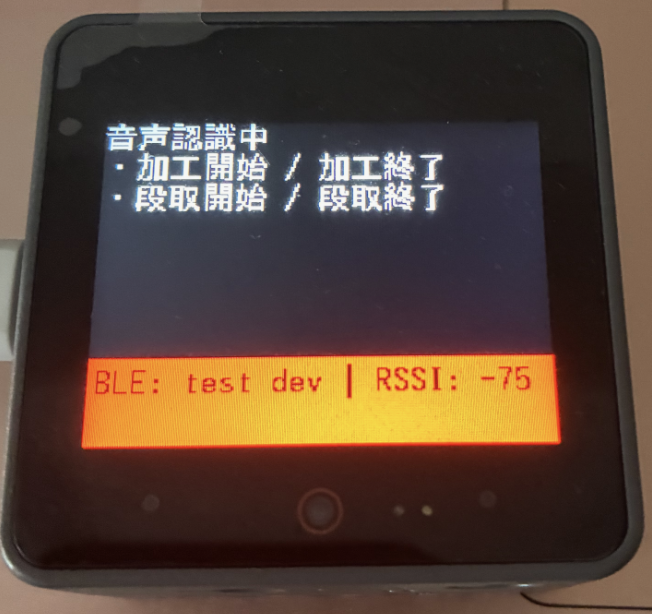
\includegraphics[width=\linewidth]{recording.png}
    \par{\scriptsize (b) 音声認識中の画面}
    \vspace{2mm}
    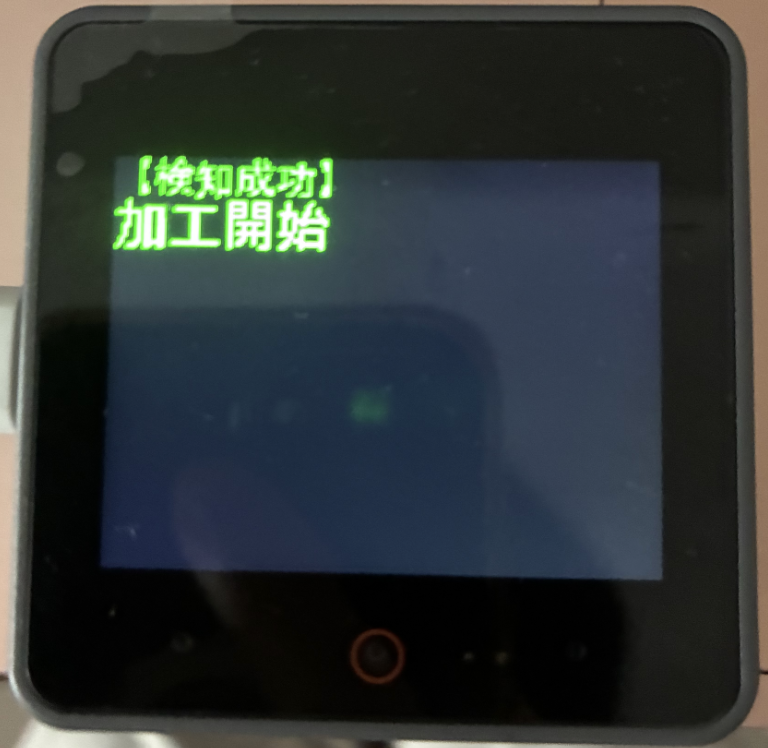
\includegraphics[width=\linewidth]{recognized.png}
    \par{\scriptsize (c) 検知成功の画面}
  \end{minipage}
  \caption{提案システムの構成と端末画面}
  \label{fig:system}
\end{figure}

\section{研究内容}
\subsection{システム構成}
図\ref{fig:system}にシステム構成と端末画面を示す。
M5CoreS3は、BLEタグの接近時に音声を録音し、Wi-Fiでサーバへ送信する。
サーバではWhisperで音声をテキスト化する\cite{radford2022whisper}。
GPT-4で作業カテゴリを抽出し、JSON形式に構造化する\cite{openai2023gpt4}。
対象は「加工開始」「加工終了」「段取開始」「段取終了」の4種類とする。
図\ref{fig:system}(b)では対象フレーズとRSSIを表示する。
図\ref{fig:system}(c)では「加工開始」の検知結果を表示する。
ログは作業カテゴリ、時刻、工作機械IDで構成する。
工作機械IDは設置端末との対応付けから取得する。
データベースへの蓄積とWeb画面での可視化は、今後の実装対象とする。

\subsection{BLE近接判定と録音制御}
BLEスキャンと音声処理を並行して実行する。
接近判定にはRSSIの移動平均を用い、一時的な変動を抑える。
接近中に一定以上の音が150 ms続くと録音を開始する。
無音が400 ms続くと終了する。
頭切れを防ぐため、開始前400 msの音声も含める。
ただし、音量による検出では発話と騒音を区別できず、BLEによる接近判定だけでは発話者を識別できない。

\section{現在の進捗と動作確認結果}
BLEスキャン、接近判定、録音制御、およびサーバ連携を実装した。
WhisperとGPT-4による解析処理を構築し、端末で「加工開始」の検知成功表示を確認した。
予備確認での応答時間は2.5～4.0秒であった。
測定条件と試行回数は未整理のため、参考値とする。
工場での認識精度と負担軽減効果は未評価である。

\section{今後の計画}
\begin{enumerate}
  \item \textbf{近接判定の調整}\quad
  現場のRSSIから移動平均の窓幅と閾値を調整する。
  接近・離脱の閾値の分離や動的変更を検討する。
  作業者の向きや遮蔽物による電波強度の変化も確認する。
  接近判定の安定性と録音開始の遅れの両面から条件を決める。

  \item \textbf{騒音・対象外発話への対策}\quad
  軽量なVADの検出性能と処理負荷を評価する。
  対象外発話の「該当なし」判定とJSONの値検証を導入する。
  金属打撃音や機械の稼働音、第三者の会話を含む条件で検証する。
  出力形式の妥当性と作業カテゴリの正確さは別々に評価する。
  ノイズ低減処理はVADとは分けて必要性を検討する。

  \item \textbf{ログ蓄積と現場評価}\quad
  作業カテゴリ、時刻、工作機械IDを蓄積するデータベースとWeb画面を構築する。
  開始・終了ログから作業時間を算出する。
  作業者IDの記録には、BLEタグと作業者の対応付けを導入する。
  近接判定の有無で誤記録率を比較し、認識成功率、取りこぼし率、応答時間、記録負担を評価する。
  手書きや端末入力と比較し、記録に要する時間と作業の中断回数を調べる。
  評価では4種類のフレーズを同数ずつ発声する。
  作業者と端末の距離、騒音条件、試行回数を記録する。
  誤記録と取りこぼしを分けて集計し、接近判定と音声解析のどちらに改善が必要かを検討する。
\end{enumerate}

\begingroup
\small
\bibliographystyle{junsrt}
\bibliography{references}
\endgroup
\end{document}
